\begin{figure}[h!]
	\centering
	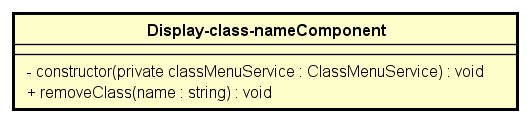
\includegraphics[scale=0.8]{res/sections/SpecificaFrontEnd/Components/Disegnetti/display-class-name.png}
	\caption{Diagramma della classe Display-class-name}
\end{figure}

\begin{itemize}
	\item \textbf{Descrizione:}\\
	Serve per mostrare il nome della classe.
	\item \textbf{Utilizzo:}\\
	Viene utilizata da EditClassMenuComponent per visualizzare i nomi delle classi.
	\item \textbf{Metodi:}
		\begin{itemize}
			\item \emph{-constructor(private classMenuService: ClassMenuService)}\\
    		Costruttore della classe\\
    		\textbf{Parametri:}
    		\begin{itemize}
    			\item \emph{classMenuService: ClassMenuService}\\
    			Crea un istanziazione di ClassMenuService
    		\end{itemize}
    		\item \emph{+removeClass(name: string)}\\
    		Rimuove la classe selezionata\\
    		\textbf{Parametri:}
    		\begin{itemize}
    			\item \emph{name: string}\\
    			Nome della classe da eliminare
    		\end{itemize}
		\end{itemize}
\end{itemize}